\section{The Large Hadron Collider at CERN}%
\label{sec:lhc}

The LHC~\cite{Evans:2008zzb} is a proton and heavy-ion collider experiment
located at CERN\footnote{From the French \emph{Conseil Européen pour la
    Recherche Nucléaire} referring to both the research organisation and the
  location of the laboratory sites.} at the French--Swiss border in Geneva,
Switzerland. At present, the LHC is the world's highest-energy, laboratory-based
particle collider experiment with proton beam energies of up to \SI{6.8}{\TeV}
and proton--proton (\pp) centre-of-mass energies, $\sqrt{s}$, of up to
\SI{13.6}{\TeV}. The focus of this section lies on the operation of the LHC
using beams of protons.

The LHC was constructed in the former tunnel of the CERN Large Electron-Positron
Collider (LEP) with a circumference of \SI{26.7}{\kilo\metre}, first becoming
operational in 2008. It is a synchrotron consisting of two counter-rotating
beams of protons that are accelerated using alternating electric fields in
superconducting radio frequency resonators/cavities. The beams are bent into a
cyclic trajectory around the ring using superconducting dipole magnets with
field strengths of about \SI{8}{\tesla}. Along the ring, numerous quadrupole
magnets are used for controlled focusing and defocusing of the proton beams.
% Synchrotron: 1232 dipoles (superconducting) -> Magnetic field of
% \SI{8.3}{\tesla} required for \SI{7}{\TeV} beam energy operation

To reach proton energies necessary for the injection into the LHC, the
infrastructure of the CERN accelerator complex is used, which is schematically
depicted in~\Cref{fig:cern_accelerator_complex}. Protons are first accelerated
in LINAC 2\footnote{Short for \textbf{lin}ear \textbf{ac}celerator.}, the Proton
Synchrotron Booster (BOOSTER), the Proton Synchrotron (PS), and finally in the
Super Proton Synchrotron (SPS) after which the beams are injected into the LHC
with proton energies of \SI{450}{\GeV}~\cite{Evans:2008zzb}. The protons are
further accelerated in the LHC until the target energy is reached. At this
point, the beams are brought into collision at four points, the interaction
points (IPs), along the ring. Four large experiments are situated at these IPs
to observe and record particle collision events at the LHC:
ATLAS~\cite{PERF-2007-01}, CMS~\cite{CMS-CMS-00-001},
ALICE~\cite{ALICE:2008ngc}, and LHCb~\cite{LHCb:2008vvz}. The ATLAS and CMS
experiments are particle detector experiments targeting extensive physics
programmes, while the ALICE and LHCb are more specialised experiments. The ALICE
experiment studies the production of the quark-gluon plasma, a state of matter
with asymptotically free quarks and gluons occurring at temperatures similar to
those right after the Big Bang, in heavy-ion collisions. The LHCb experiment
investigates the nature the observed matter-antimatter asymmetry in the universe
by studying CP violation in decays of hadrons containing $b$-quarks. Several
smaller experiments are installed at the LHC to study physics processes at small
angles with respect to the beamline of the LHC, or exotic, possibly long-lived,
particles. Such experiments are, for example, LHCf~\cite{LHCf:2008lfy},
TOTEM~\cite{TOTEM:2008lue}, MoEDAL~\cite{MoEDAL:2009jwa}, or
FASER~\cite{FASER:2019aik}.

\begin{figure}[htbp]
  \centering

  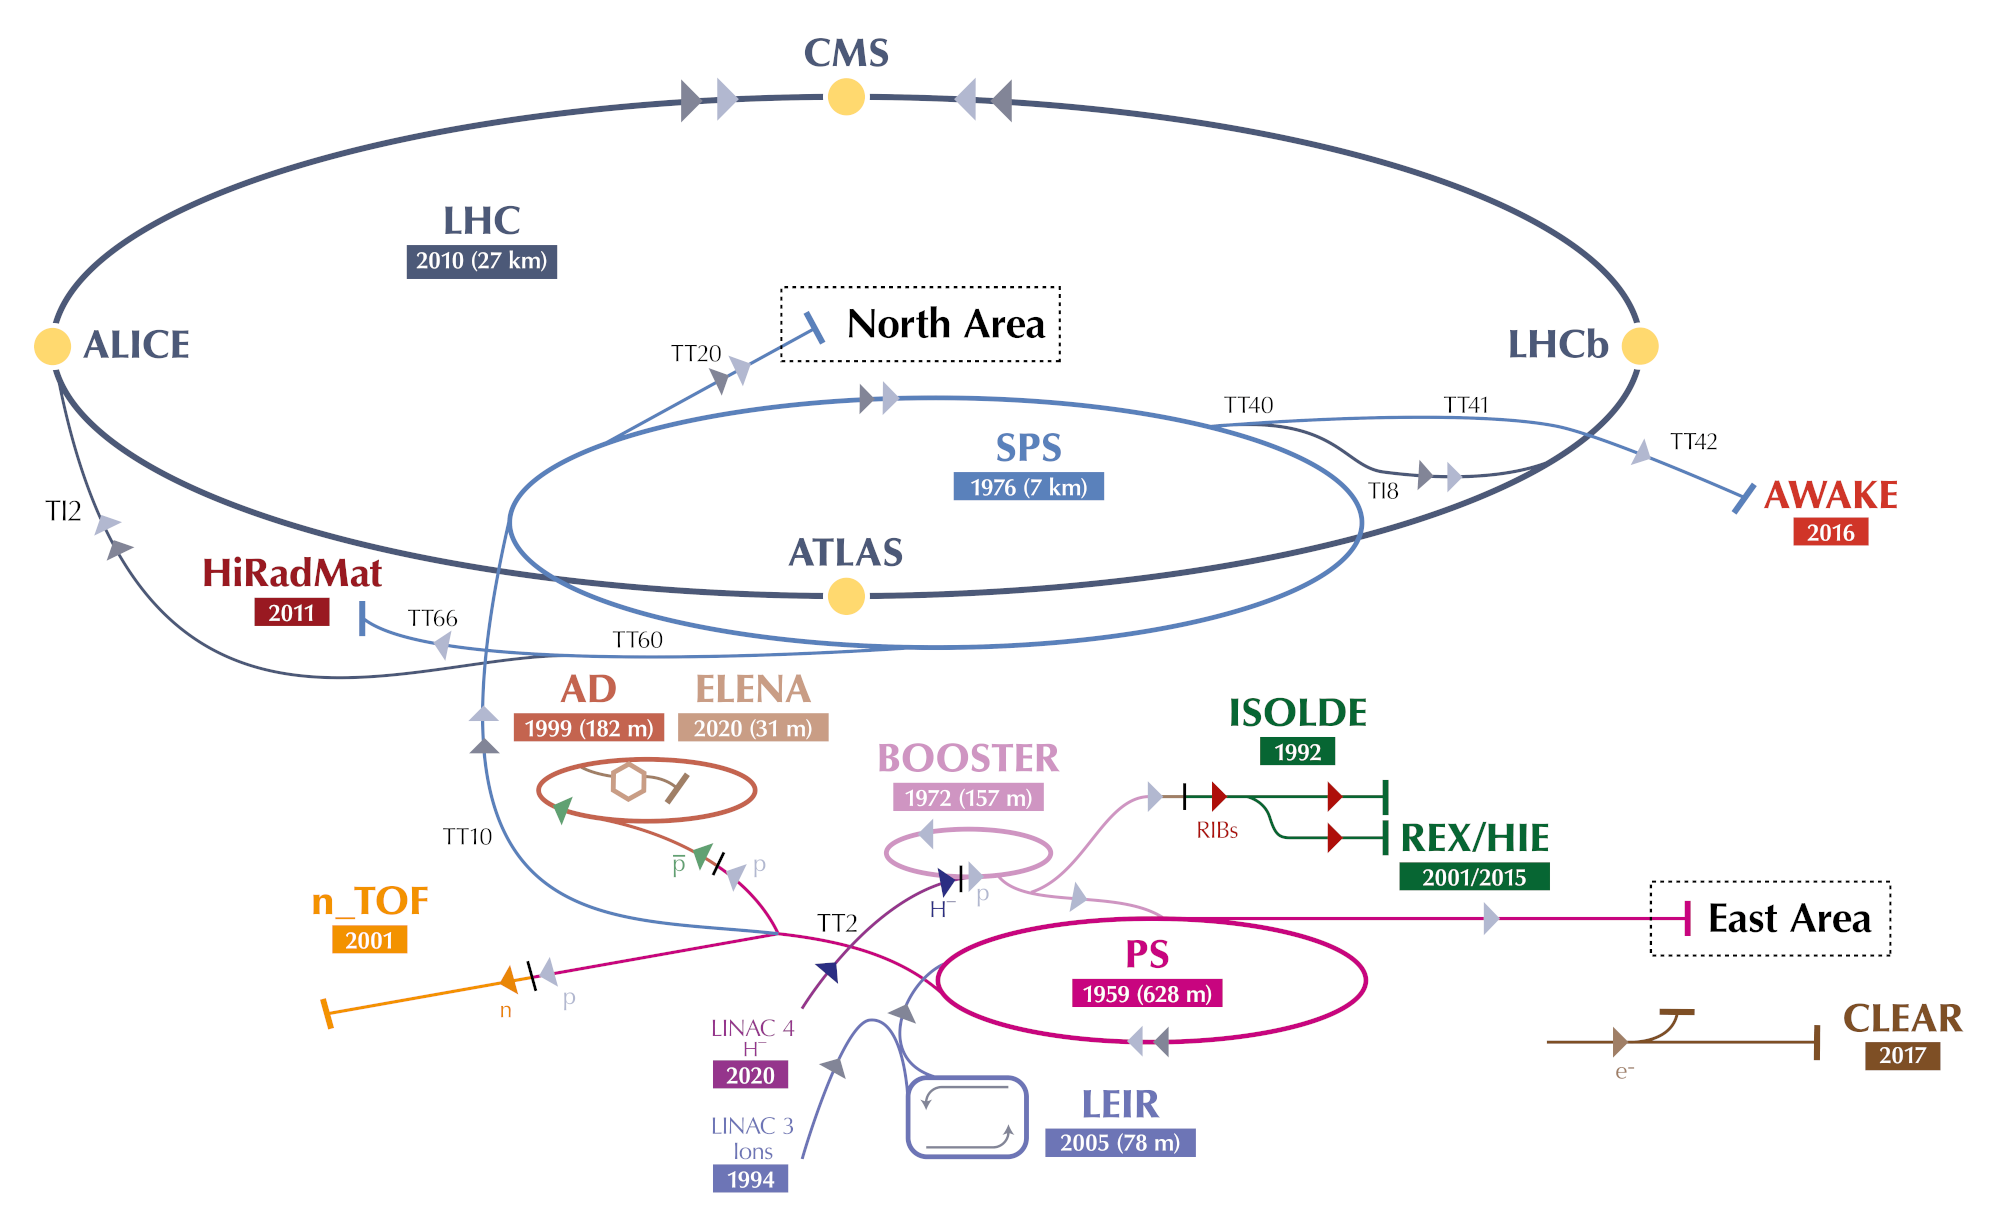
\includegraphics[width=0.9\textwidth, trim=10.5cm 44cm 2cm 20cm,
  clip]{lhc/cern_complex}

  \caption{The CERN accelerator complex in August 2018. The image is adapted
    from Ref.~\cite{Mobs:2684277}.}%
  \label{fig:cern_accelerator_complex}
\end{figure}

Operational history.

Particle collision events are recorded and reconstructed using the ATLAS
detector, which is one of two general-purpose particle detector experiments at
the LHC.

Centre of mass energy and instantaneous / integrated luminosity.

% - Energy to produce Higgs boson pairs can, at present, not be achieved with
%   electron positron colliders -> VHH production which would require CMS in excess of 300 GeV

% - Cross section of HH production - Ndot = L * sig
% - LHC proton and heavy-ion collider, though exclusively working with \pp
% collision data.

\begin{itemize}
\item Two proton beams circulating in opposite directions. In bunches. What are
  bunches? -> Symmetric

\item Provides high-energy particle collisions for four large scale experiments:
  Smaller experiments?

\item What is the goal of the LHC? -> energy frontier (protons instead of
  electrons due to reduced synchrotron radiation)

\item Run history (time?): Run 1 \SI{7}{\TeV} (2010--2011) / \SI{8}{\TeV}
  (2012); Run 2 \SI{13}{\TeV} (2015--2018); Run 3 \SI{13.6}{\TeV} (2022--)
  commenced in 2022 and, at present, is forseen to end in 2026.

\item Performance characteristics of the \pp operation of the LHC during Run~2:

  \begin{itemize}
  \item Bunches \& Bunch spacing: 2556 (\SI{25}{\nano\second}) -- but 2808 RF
    buckets (not all filled)
  \item Protons per bunch: \num{1.1e11}
  \item Luminosity: \SI{2.1e34}{\per\centi\metre\squared\per\second} (design:
    \SI{1.0e34}{\per\centi\metre\squared\per\second})
  \item $\sqrt{s} = \SI{13}{\TeV}$
  \item Pile-up?
  \item Delivered integrated luminosity: about \SI{160}{\ifb}
    \end{itemize}

\item How is the luminosity of a collider calculated?

\item How does Luminosity relate to event rate / pile-up?
  \begin{align*}
    \frac{\mathrm{d}N}{\mathrm{d}t} = L \sigma
  \end{align*}
  Inelastic \pp cross-section at $\sqrt{s} = \SI{13}{\TeV}$ ca.\
  \SI{80}{\milli\barn}~\cite{STDM-2015-05}.

\end{itemize}

% Luminosity or pile-up plots?
% https://twiki.cern.ch/twiki/bin/view/AtlasPublic/LuminosityPublicResultsRun2

\begin{figure}[htbp]
  \centering

  \begin{subfigure}{0.47\textwidth}
    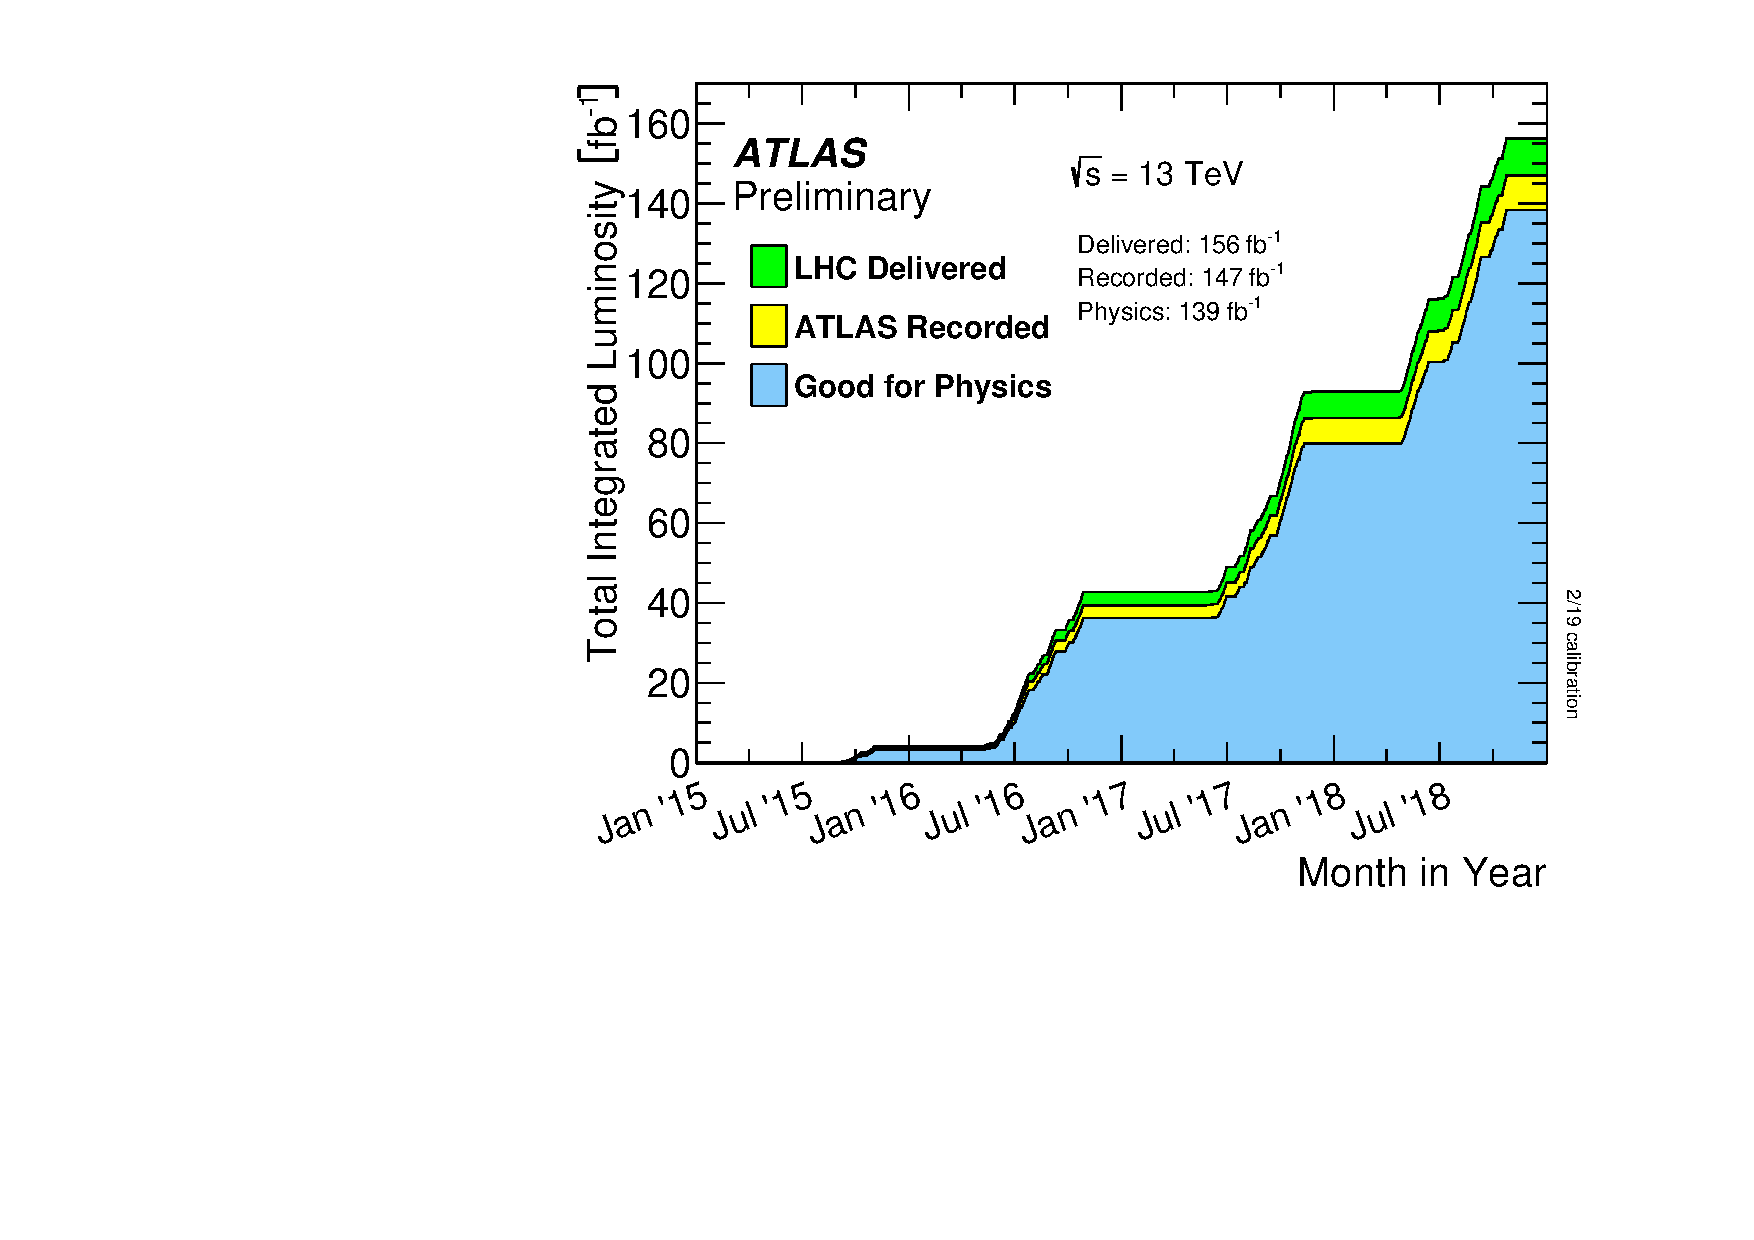
\includegraphics[width=\textwidth]{lhc/int_lumi_vs_time}
    \subcaption{}
  \end{subfigure}\hspace*{0.02\textwidth}%
  \begin{subfigure}{0.47\textwidth}
    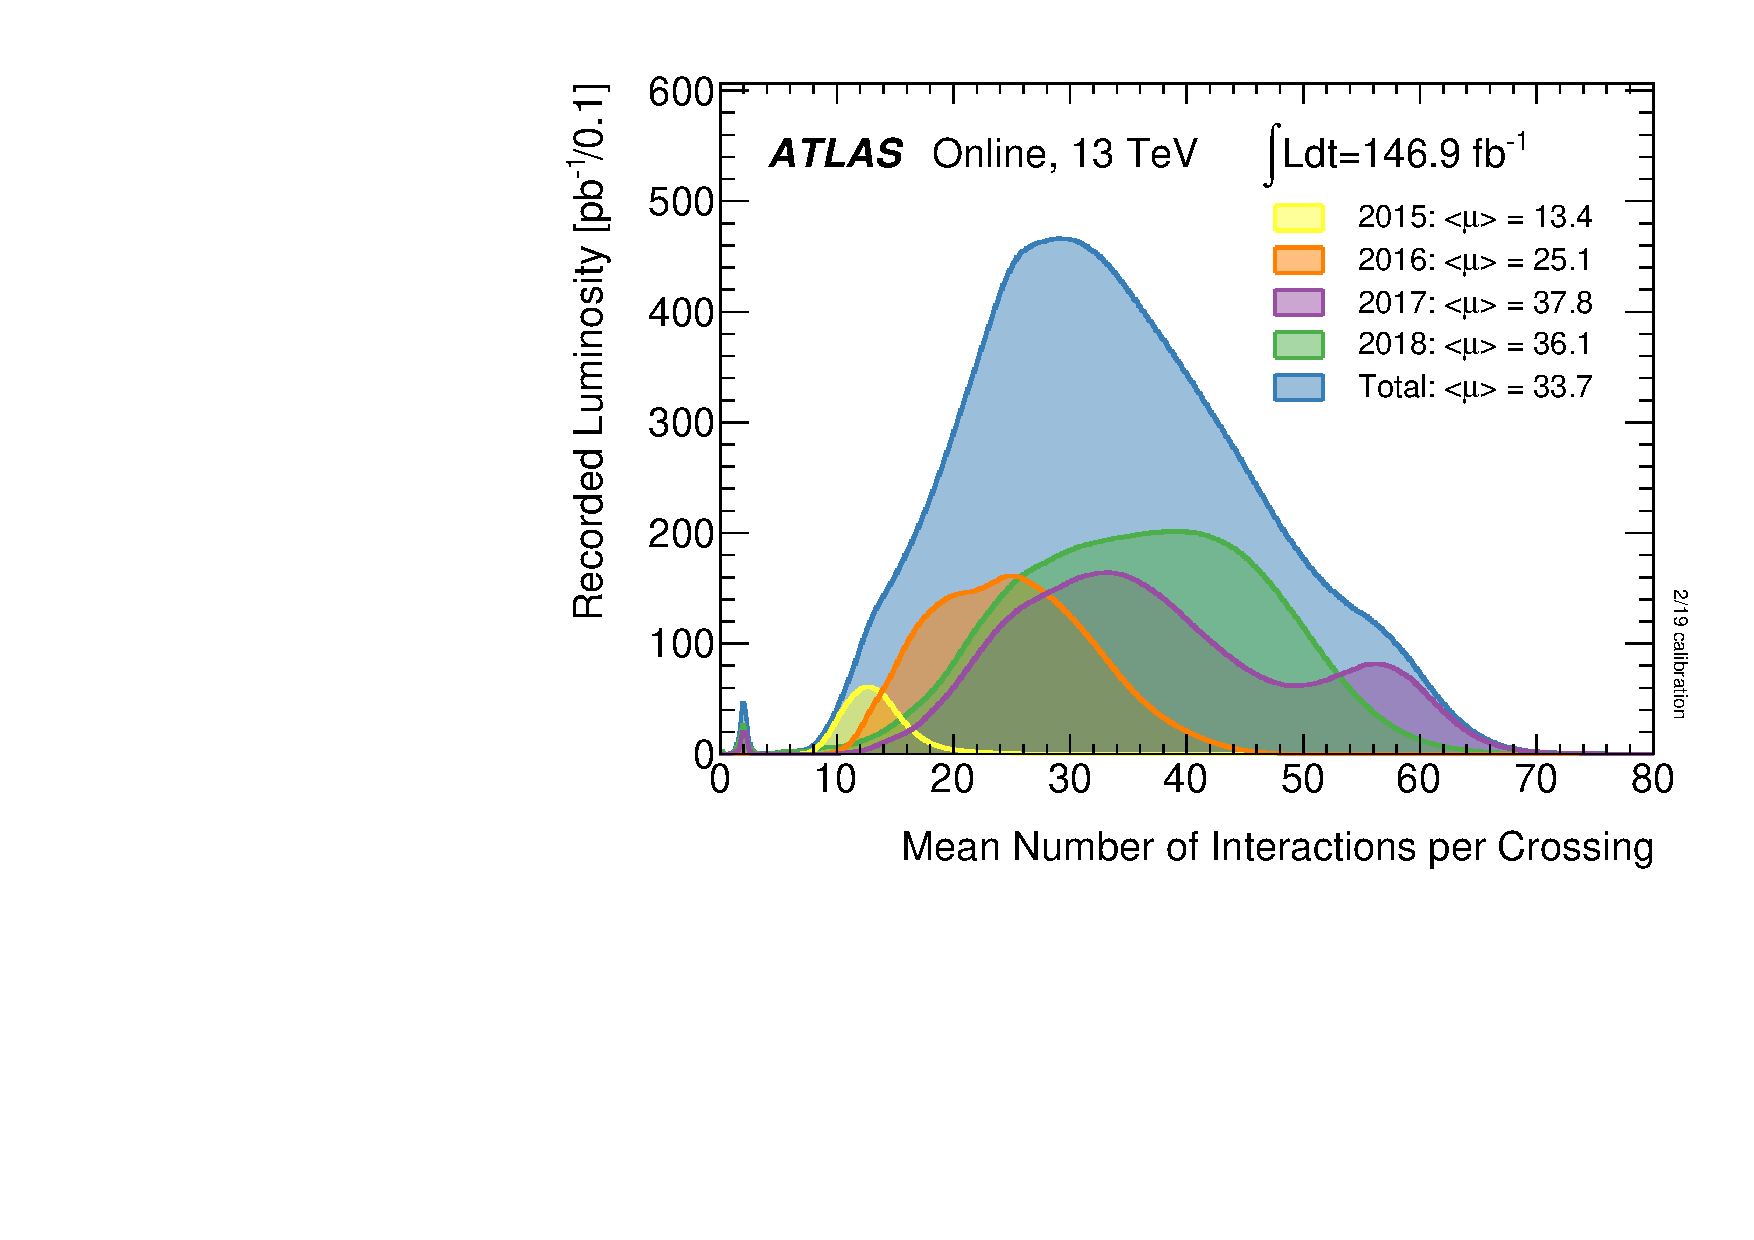
\includegraphics[width=\textwidth]{lhc/mu_2015_2018}
    \subcaption{}
  \end{subfigure}

  \caption{The integrated luminosity as a function of time (a) and the
    luminosity-weighted mean number of interactions per bunch-crossing (b) of
    LHC in \pp operation mode during Run~2. In figure (a), the integrated
    luminosity delivered by the LHC (green), recorded by the ATLAS detector
    (yellow), and the integrated luminosity of the \pp-collision dataset passing
    the data-qualtiy criteria~\cite{DAPR-2018-01} of the ATLAS collaboration
    (blue) is shown. The mean number of interactions per bunch-crossing, $\mu$,
    is calculated from the instantaneous luminosity assuming an inelastic \pp
    cross-section at $\sqrt{s} = \SI{13}{\TeV}$ of \SI{80}{\milli\barn}. The
    figures are taken from~\cite{atlas_luminosity_summary_plots}.}%
  \label{fig:lumi_and_pu}
\end{figure}

%%% Local Variables:
%%% mode: latex
%%% TeX-master: "../../phd_thesis"
%%% End:
